\lesson{5}{Oct 14 2021 Thu (08:29:41)}{Honors Electrons}{Unit 2}

\subsubsection*{What are the quantum numbers that describe probable electron location?}

\begin{definition}[Principal Quantum Number (n)]
    The Principal Quantum number describes the energy level within an atom.
    Positive whole numbers, from one to infinity, are used to represent energy
    levels. These numbers are used to represent energy levels in electron
    configurations and orbital notation.

    \begin{align}
        1s^{2}2s^{2}2p^{2}
    \end{align}
\end{definition}

\begin{definition}[Angular Momentum Quantum Number (l)]
    An electron needs both the \bf{principal number} and the \bf{angular
    momentum quantum number} to identify its specific sublevel. The angular
    momentum quantum number describes the type of sublevel
    ($s, p, d, f, \ldots$) using a number instead of a letter
    ($l = 0, 1, 2, 3, \ldots$).

    Basically, electrons in the $2s$ subshell can also be described as
    
    $n = 2, l = 0$ using quantum numbers. It's two different ways of describing
    the same probable positions for electrons. The principal quantum number $n = 2$
    means it's in the second energy level of the atom. The number $l = 0$ tells
    you that the electron is found in an $s$ sublevel.
    
    Let's use the element chlorine as an example. Chlorine has 17 total
    electrons. It has an electron configuration of:

    \begin{align}
        1s^{2}2s^{2}2p^{6}3s^{2}3p^{5}
    \end{align}
    
    What are the first $2$ quantum numbers for the $6$ electrons in the $2p$ subshell?

    \begin{align}
        n = 2, l = 1
    \end{align}

    The energy level is $2$, and  the $p$ subshell is represented by $l = 1$.
\end{definition}

\begin{definition}[Magnetic Quantum Number ($m_l$)]
    The \bf{magnetic quantum number ($m_l$)} represents the specific orbital an
    electron is likely to occupy. Each type of sublevel has a specific number of
    orbitals, and each orbital can hold two electrons.

    The range of magnetic quantum numbers for a given sublevel ($1$) is from $-1$ to
    $+1$. For example, in an $s$ sublevel ($l = 0$) there is only one available
    orbital.

    It has a \bf{Magnetic Quantum Number} of $m_l = 0$. A $p$ sublevel ($l = 1$)
    has $3$ orbitals with \bf{Magnetic Quantum Numbers} of $m_l = -1, -, +1$.

    \begin{align}
        n = 2, l = 1, m_l = -1, 0, +1
    \end{align}
    
    The magnetic quantum number is $-1, 0$ and $+1$
    because the $p$ subshell consists of $3$ orbitals that can hold electrons.
\end{definition}

\begin{definition}[Spin Quantum Number ($m_s$)]
    The combination of:
    
    \begin{itemize}
        \item Principal
        \item Angular Momentum
        \item Magnetic Quantum Numbers
    \end{itemize}
    
    identifies the location of an electron by:
    
    \begin{itemize}
        \item Energy Level
        \item Sublevel
        \item Orbital
    \end{itemize}
    
    Each orbital can hold $2$ electrons, so $2$ electrons in the same
    orbital would share the same values for the first $3$ quantum numbers. A
    $4th$ quantum number, called the \bf{spin quantum number} ($m_s$), is
    needed to identify the specific electron within an orbital. It represents
    the spin direction of an electron on its axis.

    According to Hund's second rule, two negatively charged electrons located
    near each other in the same orbital area are most stable when they spin in
    opposite directions. There are only $2$ choices for the spin quantum number:

    \begin{align}
        +\frac{1}{2} \rm{OR} -\frac{1}{2}
    \end{align}

    An electron can only be assigned $1$ spin quantum number. These two values
    represent the two different directions an electron can spin on an imaginary
    axis.

    Let's give it a shot.

    Chlorine has $17$ total electrons. It has an electron configuration of:
    
    \begin{align}
        1s^{2}2s^{2}2p^{6}3s^{2}3p^{5}
    \end{align}
    
    Which quantum numbers represent the probable location and
    motion of an electron in the $2p$ subshell and orbital $m_i = 0$?

    \begin{align}
        n = 2, l = 1, m_l = 0, m_s = +\frac{1}{2} \rm{OR} -\frac{1}{2}
    \end{align}

    The spin number is $+\frac{1}{2} \rm{OR} -\frac{1}{2}$ because $m_l = 0$
    orbital holds $2$ electrons. The answer could refer to either electron
    within the orbital. However, the spin quantum number can only be assigned to
    $1$ electron in the orbital, not both. Therefore, the answer could be:

    \begin{align}
        n = 2, l = 1, m_l = 0, m_s = +\frac{1}{2} \\
        \rm{OR} \\
        n = 2, l = 1, m_l = 0, m_s = -\frac{1}{2} \\
    \end{align}
\end{definition}

\subsubsection*{How do orbital notation diagrams model electron arrangements within an atom?}

Negatively charged electrons repel each other, so they spread out as much as
possible within the orbitals of a given sublevel. This is described by \bf{Hund's
first rule}, which stats:

\begin{quote}
    The lowest energy atomic state is the one that maximizes the total spin quantum number for the electrons in the open subshell
\end{quote}

\begin{marginfigure}
    \centering
    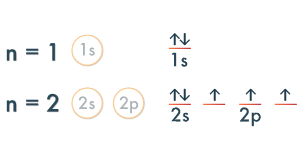
\includegraphics[width=\textwidth,height=\textheight,keepaspectratio]{images/hund-first-rule}
    \sidecaption{Hund's first rule.}
    \label{fig:hund-first-rule}
\end{marginfigure}

This atom has $7$ electrons. Each orbital is represented by a line and the
energy level and sublevel is shown below the line. Each electron is represented
by an arrow. $2$ Electrons can be placed in the level $1s$ and $2s$ subshells. Each
of the two electrons is represented by an arrow. One is pointed up to show a
clockwise spin, and the other is shown pointing down to indicate a
counterclockwise spin. According to Hund's second rule, $2$ electrons in the
same orbital will spin in opposite directions to reduce the repulsion of the
electrons.

\subsubsection*{How do the electrostatic forces between electrons influence their orbital spin?}

Electric charge is a physical property of matter that causes a particle to
experience a force when interacting with other charged particles. These
electrostatic forces create an electric field that attracts or repels other
charged particles.

The pattern of lines in the images below are called electric field lines. These
lines point in the direction another positive charge would follow if placed on
these lines.

\begin{marginfigure}
    \centering
    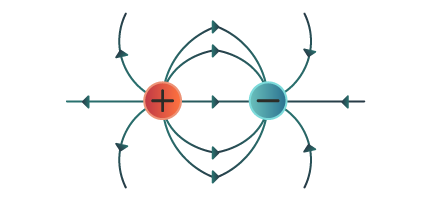
\includegraphics[width=\textwidth,height=\textheight,keepaspectratio]{images/attracted-atoms}
    \caption{Particles with opposite charges attract one another. The electric
    field lines are directed away from the positively charged particle toward
    the negatively charged particle.}
    \label{fig:attracted-atoms}
\end{marginfigure}

\begin{marginfigure}
    \centering
    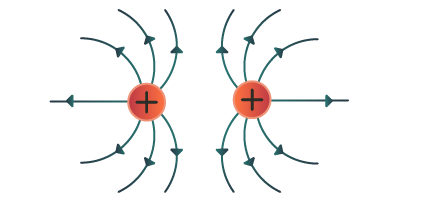
\includegraphics[width=\textwidth,height=\textheight,keepaspectratio]{images/repeled-atoms}
    \caption{Two particles with the same charge repel each other. The electric
    field lines of each positively charged particle are directed away from one
    another.}
    \label{fig:repeled-atoms}
\end{marginfigure}

Electric charge can be neither created nor destroyed. The total amounts of
positive charges and negative charges in the universe are always equal, creating
a neutral net charge of $0$.

\paragraph{Inside the Atom} The electrostatic forces between tiny subatomic
particles are relatively enormous. The repulsive forces between electrons and
the attractive forces between electrons and protons is so significant, it
influences the arrangement of electrons within energy levels, subshells, and
individual orbitals. It also affects electron spin, preventing two electrons
from spinning in the same direction within the same orbital. Instead, electrons
within the same orbital spin in opposite directions from one another.

\begin{marginfigure}
    \centering
    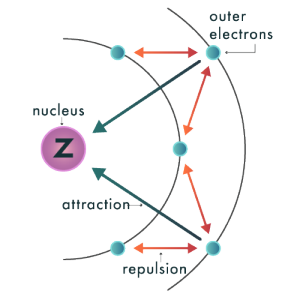
\includegraphics[width=\textwidth,height=\textheight,keepaspectratio]{images/inside-the-atom}
    \caption{This is what it looks like inside the atom.}
    \label{fig:inside-the-atom}
\end{marginfigure}

\paragraph{Between Atoms} In a neutral atom, the number of positively charged
particles (protons) equals the number of negatively charged particles
(electrons). Therefore, the net charge on the atom is $0$.

If an electron moves from one neutral atom to another, two charged atoms are
created. The first atom loses one electron, and so it acquires a $+1$ charge. The
second atom gains one electron, so it acquires a $-1$ charge.

\subsubsection*{How is the strength of an electrostatic force determined?}

The relationship that explains the force between charged particles was
discovered by Charles Coulomb in the 18th century. He discovered that electric
force decreases inversely as the square of the distance between charges. This is
referred to as Coulomb's law.

Basically, as the distance between charged particles decreases, the force
between them increases, and vice versa. Also, an increase of electrical charge
increases the electrostatic forces between them. A decrease in electrical charge
decreases the electrostatic forces between them.

\begin{definition}[Coulomb's Law of Electrical Forces]
    The force between two charges is directly proportional to the product of the
    charges and inversely proportional to the square of the separation distance.
    The force between particles acts along a straight line from one charge to
    the other.

    \begin{align}
        F = \frac{kq_1q_2}{d^2}
    \end{align}

    $F$ = The electrical force between the two charges, measured in Newtons.
    $k$ = $8.99 \times 10^9 \frac{Nm^2}{C^2}$.
    $q_1$ = Quantity of charge of one particle, measured in coulombs.
    $q_2$ = The quantity of charge of the second particle, measured in coulombs.
    $d^2$ = The distance between the objects squared, measured in meters.
\end{definition}

\paragraph{Nuclear Charge} According to Coulomb's law, charged particles that
are closer to one another or have a larger product of electrical charge will
experience stronger electrostatic forces. This is certainly true when it comes
to the interactions between electrons and the nucleus. The net positive charge
associated with the protons inside the nucleus of an atom is referred to as its
nuclear charge. Electrons closer to the nucleus in energy level n = 1 will have
a stronger attraction toward the nucleus due to its nuclear charge. This means
it will take more energy to move electrons closest to the nucleus from their
orbital regions. Remember, electrons will jump to higher levels with the
addition of energy. But those closest to the nucleus have strong electrostatic
forces holding their position.

\begin{marginfigure}
    \centering
    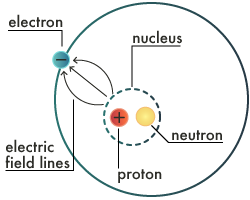
\includegraphics[width=\textwidth,height=\textheight,keepaspectratio]{images/nuclear-charge}
    \caption{This what it looks like when an atom has a nuclear change.}
    \label{fig:nuclear-change}
\end{marginfigure}

\newpage
